\documentclass[12pt]{extarticle}
\usepackage[english]{babel}
\usepackage{graphicx}
\usepackage{framed}
\usepackage{amsmath}
\usepackage{amssymb}
\usepackage{amsfonts}
\usepackage{enumerate}
\usepackage[utf8]{inputenc}
\usepackage[top=1 in,bottom=1in, left=1 in, right=1 in]{geometry}

\title{Task 1}
\author{s1703913}
\date{April 2019}

\begin{document}

\maketitle
\pagebreak

\section{Task 1.1}
\begin{figure}[h!]
\caption{First ten samples in the training data (Xtrn) for Class k (k=1,...,10).}
\centering
\includegraphics[trim={2cm 7cm 2cm 7cm},height=4cm,width=4cm]{task1_1_imgs_class1}
\includegraphics[trim={2cm 7cm 2cm 7cm},height=4cm,width=4cm]{task1_1_imgs_class2}
\includegraphics[trim={2cm 7cm 2cm 7cm},height=4cm,width=4cm]{task1_1_imgs_class3}
\includegraphics[trim={2cm 7cm 2cm 7cm},height=4cm,width=4cm]{task1_1_imgs_class4}
\includegraphics[trim={2cm 7cm 2cm 7cm},height=4cm,width=4cm]{task1_1_imgs_class5}
\includegraphics[trim={2cm 7cm 2cm 7cm},height=4cm,width=4cm]{task1_1_imgs_class6}
\includegraphics[trim={2cm 7cm 2cm 7cm},height=4cm,width=4cm]{task1_1_imgs_class7}
\includegraphics[trim={2cm 7cm 2cm 7cm},height=4cm,width=4cm]{task1_1_imgs_class8}
\includegraphics[trim={2cm 7cm 2cm 7cm},height=4cm,width=4cm]{task1_1_imgs_class9}
\includegraphics[trim={2cm 7cm 2cm 7cm},height=4cm,width=4cm]{task1_1_imgs_class10}
\end{figure}
\pagebreak

\section{Task 1.2}
\begin{figure}[h!]
\caption{11 images, where image k (k=1,...,10) is the image of
   the mean vector for Class k, and image 11 is the image of the mean
   vector for all the classes.}
\centering
\includegraphics[trim={2cm 7cm 2cm 7cm},height=16cm,width=16cm]{task1_2_imgs}
\end{figure}
\pagebreak

\section{Task 1.3}
\begin{figure}[h!]
\caption{Graph of cumulative variance (NB. It is just the plot of the cumulative sum of variance for D=1,...,784. The value hasn't been normalized by the total variance.)}
\centering
\includegraphics[trim={2cm 7cm 2cm 7cm},height=16cm,width=16cm]{task1_3_graph}
\end{figure}
\pagebreak

\begin{table}[h!]
\centering
\caption{Minimum numbers of PCA dimensions to cover 70\%, 80\%, 90\%, and 95\% of the total variance.}
\begin{tabular}{ |p{3cm}|p{3cm}|  }
 \hline
 Percentage&Min. number of dimensions\\
 \hline
 70\%&26\\
 80\%&44\\
 90\%&87\\
 95\%&154\\
 \hline
\end{tabular}
\end{table}
\hfill

\section{Task 1.4}
\begin{figure}[h!]
\caption{First ten principal components, where image i (i=1,...,10) is the image of i-th principal component.}
\centering
\includegraphics[trim={2cm 7cm 2cm 7cm},height=11cm,width=11cm]{task1_4_imgs}
\end{figure}
\pagebreak

\section{Task 1.5}
\begin{figure}[h!]
\caption{Graphs of SSE where number of iterations on x-axis, SSE on y-axis for each figure.}
\end{figure}
{\centering
\includegraphics[trim={2cm 7cm 2cm 7cm},height=9cm,width=9cm]{SSEs_for_k=1}
\begin{center}
k=1 cluster
\end{center}
\includegraphics[trim={2cm 7cm 2cm 7cm},height=9cm,width=9cm]{SSEs_for_k=2}
\begin{center}
k=2 clusters
\end{center}
\includegraphics[trim={2cm 7cm 2cm 7cm},height=10cm,width=10cm]{SSEs_for_k=3}
\begin{center}
k=3 clusters
\end{center}
\includegraphics[trim={2cm 7cm 2cm 7cm},height=10cm,width=10cm]{SSEs_for_k=4}
\begin{center}
k=4 clusters
\end{center}
\includegraphics[trim={2cm 7cm 2cm 7cm},height=10cm,width=10cm]{SSEs_for_k=5}
\begin{center}
k=5 clusters
\end{center}
\includegraphics[trim={2cm 7cm 2cm 7cm},height=10cm,width=10cm]{SSEs_for_k=7}
\begin{center}
k=7 clusters
\end{center}
\includegraphics[trim={2cm 7cm 2cm 7cm},height=10cm,width=10cm]{SSEs_for_k=10}
\begin{center}
k=10 clusters
\end{center}
\includegraphics[trim={2cm 7cm 2cm 7cm},height=10cm,width=10cm]{SSEs_for_k=15}
\begin{center}
k=15 clusters
\end{center}
\includegraphics[trim={2cm 7cm 2cm 7cm},height=10cm,width=10cm]{SSEs_for_k=20}
\begin{center}
k=20 clusters
\end{center}
}

\hfill
\begin{table}[h!]
\centering
\caption{Time taken for clustering for each number of clusters k (maximum of 40 iterations).}
\begin{tabular}{ |p{3cm}|p{3cm}|  }
 \hline
 k&Time taken\\
 \hline
 1&0.31 sec\\
 2&8.62 sec\\
 3&17.27 sec\\
 4&21.18 sec\\
 5&23.10 sec\\
 7&32.45 sec\\
 10&44.50 sec\\
 15&67.09 sec\\
 20&91.62 sec\\
 \hline
\end{tabular}
\end{table}
\pagebreak

\section{Task 1.6}
\begin{figure}[h!]
\centering
\caption{Images of cluster centres obtained with k-Mean clustering k=1,2,3,4,5,7,10,15,20.}
\end{figure}
\begin{figure}[h!]
\centering
\includegraphics[trim={2cm 7cm 2cm 7cm},height=5cm,width=5cm]{task1_6_imgs_1}
\includegraphics[trim={2cm 7cm 2cm 7cm},height=5cm,width=5cm]{task1_6_imgs_2}
\includegraphics[trim={2cm 7cm 2cm 7cm},height=5cm,width=5cm]{task1_6_imgs_3}
\includegraphics[trim={2cm 7cm 2cm 7cm},height=5cm,width=5cm]{task1_6_imgs_4}
\includegraphics[trim={2cm 7cm 2cm 7cm},height=5cm,width=5cm]{task1_6_imgs_5}
\includegraphics[trim={2cm 7cm 2cm 7cm},height=5cm,width=5cm]{task1_6_imgs_7}
\includegraphics[trim={2cm 7cm 2cm 7cm},height=5cm,width=5cm]{task1_6_imgs_10}
\includegraphics[trim={2cm 7cm 2cm 7cm},height=5cm,width=5cm]{task1_6_imgs_15}
\includegraphics[trim={2cm 7cm 2cm 7cm},height=5cm,width=5cm]{task1_6_imgs_20}
\end{figure}
\pagebreak

\section{Task 1.7}
To visualize the cluster regions, I first calculated the plotting range on X and Y by moving the whole data mean M into 2D space. This gives Mx and My, after which +- 5 standard deviation is straightforward to calculate e.g. std\_x = sqrt(EVals(1)), std\_y = sqrt(EVals(2)). I then moved the 2D grid points obtained to 784 dimensions, calculated distances to clusters and assigned the minimum one to each point on the grid.

\begin{figure}[h!]
\caption{Cross section of cluster regions for k = 1,2,3,5,10.}
\centering
\includegraphics[trim={2cm 7cm 2cm 7cm},height=6cm,width=6cm]{task1_7_imgs_1}
\includegraphics[trim={2cm 7cm 2cm 7cm},height=6cm,width=6cm]{task1_7_imgs_2}
\includegraphics[trim={2cm 7cm 2cm 7cm},height=6cm,width=6cm]{task1_7_imgs_3}
\includegraphics[trim={2cm 7cm 2cm 7cm},height=6cm,width=6cm]{task1_7_imgs_5}
\includegraphics[trim={2cm 7cm 2cm 7cm},height=6cm,width=6cm]{task1_7_imgs_10}
\end{figure}
\pagebreak

\section{Task 1.8}
\begin{figure}[h!]
\caption{This is a mini research project in which I investigated the k-means clustering efficiency in terms of initial cluster centres initialization. For this I have employed SSE to measure the clustering performance. I have made 5 different experiments and have noticed how the k-means++ algorithm always comes out as the most efficient method of cluster centre initialization. On the Y axis the Sum Squared Error is represented.}
\end{figure}
{\centering
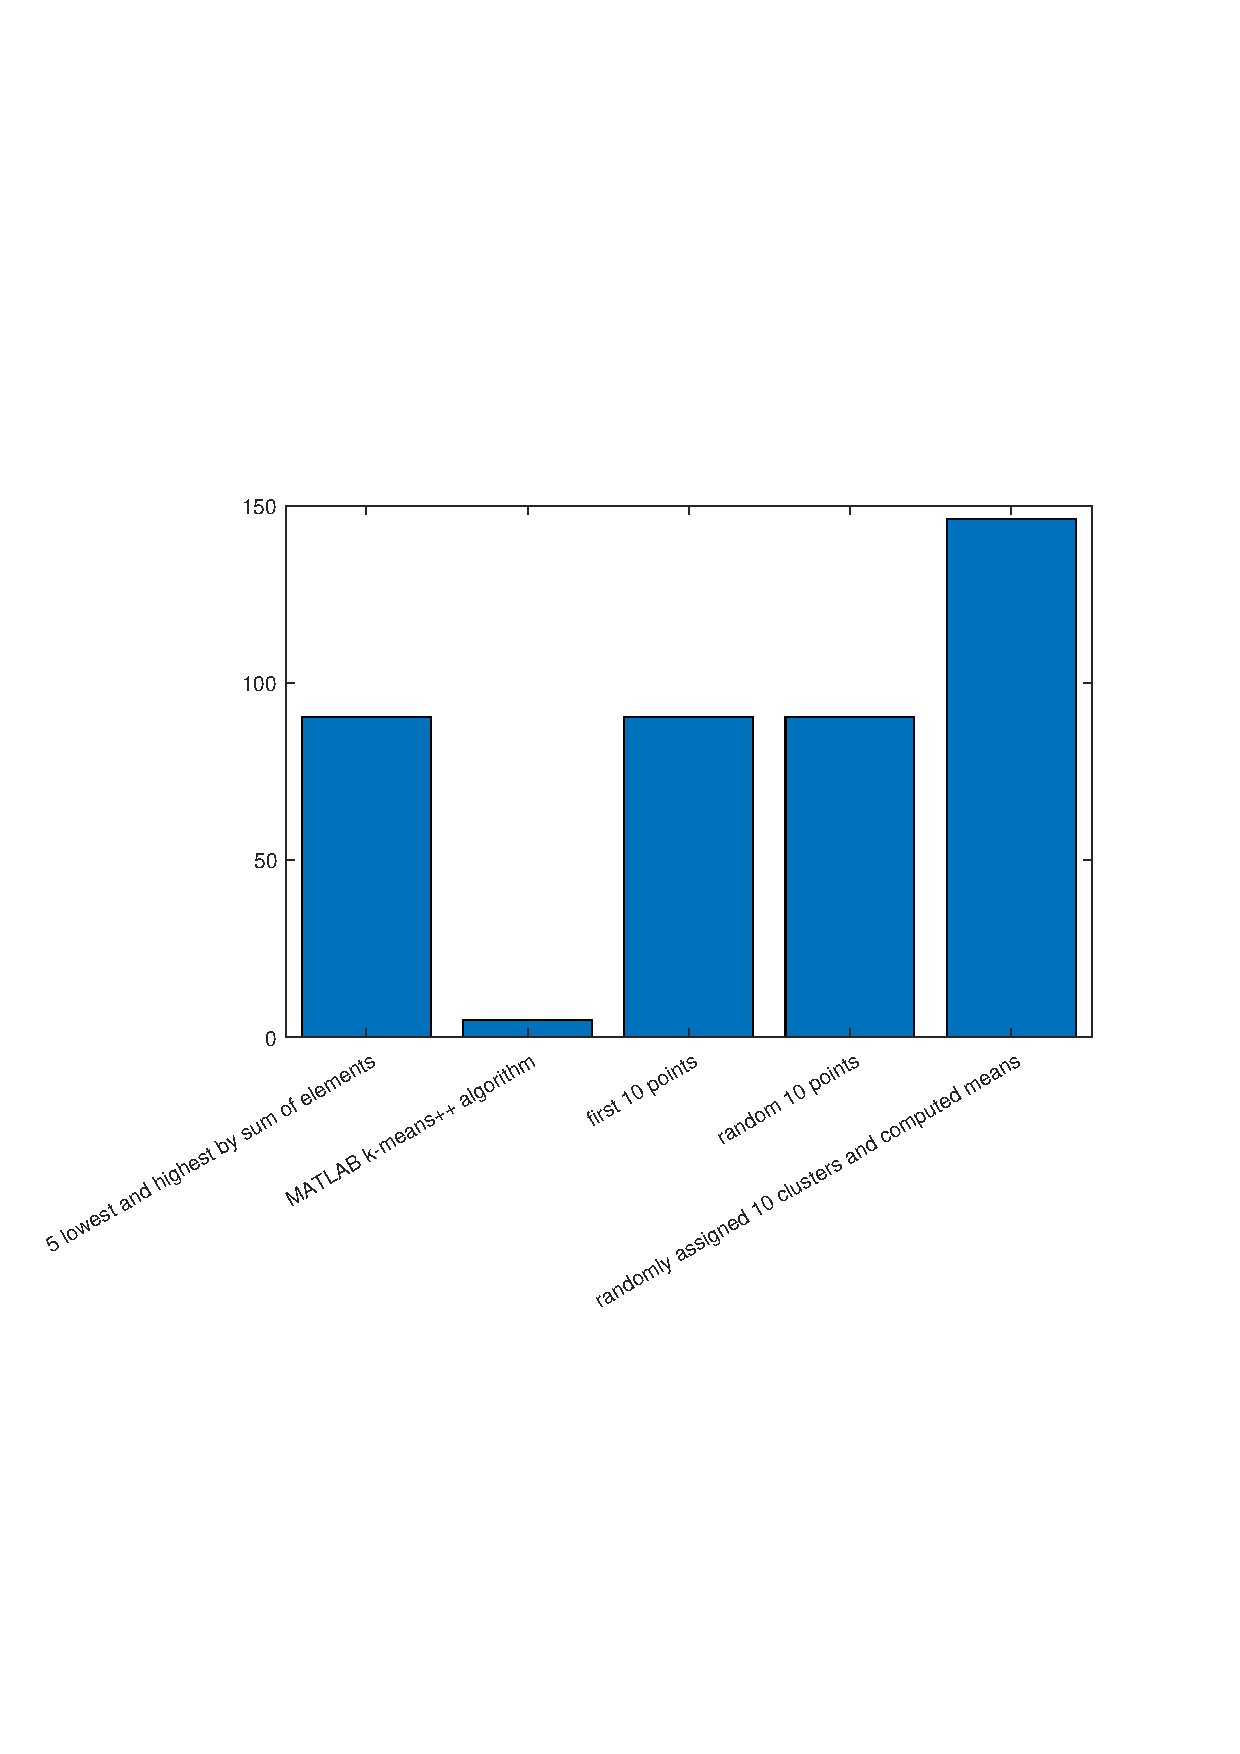
\includegraphics[trim={2cm 7cm 2cm 7cm},height=15cm,width=15cm]{task1_8_report_image_lemonorange}
\begin{center}
Cluster initialization performance on the lemonorange dataset.
\end{center}
\includegraphics[trim={2cm 7cm 2cm 7cm},height=16cm,width=16cm]{task1_8_report_image_iris}
\begin{center}
Cluster initialization performance on the iris dataset.
\end{center}
\includegraphics[trim={2cm 7cm 2cm 7cm},height=16cm,width=16cm]{task1_8_report_image_faithful}
\begin{center}
Cluster initialization performance on the faithful (volcano) dataset.
\end{center}
\includegraphics[trim={2cm 7cm 2cm 7cm},height=16cm,width=16cm]{task1_8_report_image_digits}
\begin{center}
Cluster initialization performance on the digits dataset.
\end{center}
}

\end{document}